\subsection{DNSSEC SNMP MIB implementation}
\label{section:dnssec-mib-implementation}

\subsubsection{General overview}
The OID entry point for the DNSSEC MIB is located inside the ARPA2 OID tree (enterprise OID 44469). The MIB module name is ARPA2-Experimental-DNSSEC-MIBv1 and is associated to the numerical OID \textit{.1.3.6.1.4.1.44469.666.53.46.161.1}. The path from the root down to that module is shown in Figure \ref{figure:oid-tree}.

\begin{figure}[H]
\centering
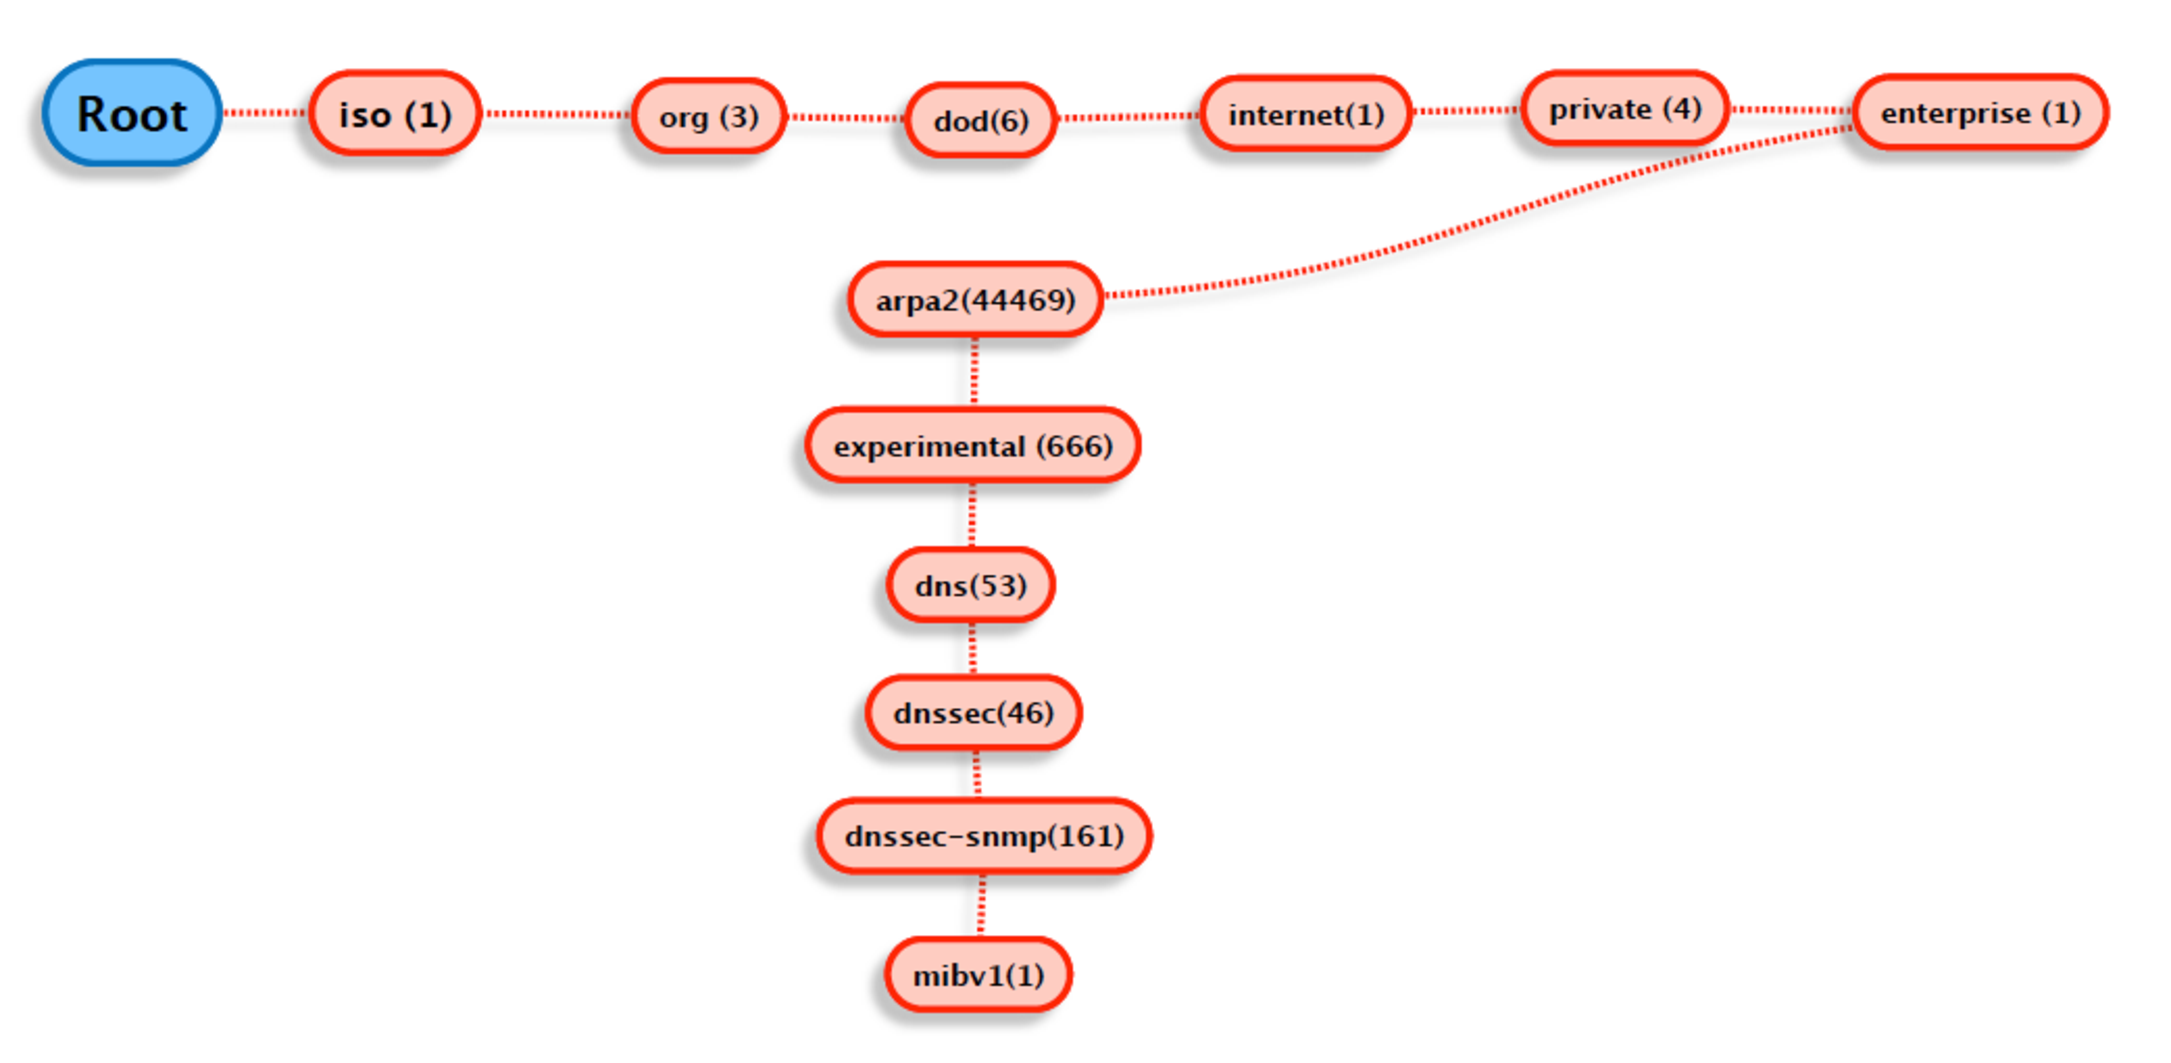
\includegraphics[scale=0.4]{Images/oid-tree.pdf}
\caption{OID Tree}
\label{figure:oid-tree}
\end{figure}


Objects defined in the MIB are organized in tables \footnote{In SNMP terminology, tables are denoted as conceptual tables or columnar objects} or scalar types. INTEGER datatypes are used to represent boolean and numeric values and data type  OCTET-STRING to represent strings (e.g domain names). Four tables are included in the MIB \textit{(dnssecZoneGlobalTable, dnssecZoneAuthNSTable, dnssecZoneSigTable, dnssecZoneDiffTable)}. To provide an easy mechanism to associate data entities to a specific zone, all MIB entries are indexed by the domain name itself (datatype OCTET-STRING).
\\
\subsubsection{Data covered by the MIB}
In section \ref{section:vital-life-signs-dnssec} are listed the most relevant parameters that need to be covered by the MIB, in order to keep track of vital life signs of DNSSEC signed zones. 
\\
The first table \textit{(dnssecZoneGlobalTable)} contains general parameters like the availability of the zone seen from the prospect of an external DNSSEC-aware resolver or the status of the signature verification of the DNSKEY RRset against the published KSK. That table also provides general data like the FQDN of the nameserver, where data is fetched from and its IP address. Furthermore entries in that table supply information about the general DNS setup for a zone. For instance, one could retrieve the information if delegations are present in a zone and subsequently check if the count of DS records matches at least the amount of delegations. 
\\
Entries in table \textit{dnssecZoneGlobalTable} are not supposed to list all data that is provided by the zone. For example, there is no need to list TTL values for each RR when the maximum and minimum TTL observed in a zone is provided. 
\\
The same applies to entries of the \textit{dnssecZoneSigTable}. Only expiration dates of essential RRs at the zone apex are covered, rather than listing each signature expiration date for every RR. For the same reason, entries in the \textit{dnssecZoneDiffTable} only provide a general indication if discrepancies between data provided by a master and slave exist. The perfect candidate to illustrate differences in a master-slave setup is the serial number of the SOA RR itself. The information if a master-slave setup exist for a particular zone can be retrieved from the \textit{dnssecZoneGlobalAuthNSCount} entry in the \textit{ dnssecZoneGlobalTable}.
\\
The general idea of the data provided in all tables in the MIB is to reflect the health status of a zone in a way that it can be easily retrieved from monitoring tools without the need of complex computations.
\\
Listing \ref{lst:snmptranslate} shows all top level elements of the created MIB including tables and their associated indexes.


\begin{listing}
\small\begin{verbatim}

+--arpa2experimentaldnssecMIBv1(1)
   |
   +--dnssecObjects(1)
   |  |
   |  +--dnssecGeneral(1)
   |  |  |
   |  +--dnssecZoneGlobal(2)
   |  |  |
   |  |  +--dnssecZoneGlobalTable(2)
   |  |     |
   |  |     +--dnssecZoneGlobalEntry(1)
   |  |        |  Index: dnssecZoneGlobalIndex
   |  |
   |  +--dnssecZoneAuthNS(3)
   |  |  |
   |  |  +--dnssecZoneAuthNSTable(3)
   |  |     |
   |  |     +--dnssecZoneAuthNSEntry(1)
   |  |        |  Index: dnssecZoneGlobalIndex
   |  |        |
   |  +--dnssecZoneSig(4)
   |  |  |
   |  |  +--dnssecZoneSigTable(4)
   |  |     |
   |  |     +--dnssecZoneSigEntry(1)
   |  |        |  Index: dnssecZoneGlobalIndex
   |  |        |
   |  +--dnssecZoneDiff(5)
   |     |
   |     +--dnssecZoneDiffTable(5)
   |        |
   |        +--dnssecZoneDiffEntry(1)
   |           |  Index: dnssecZoneGlobalIndex
   |           |
   +--dnssecMIBConformance(2)
      |
      +--dnssecMIBGroups(1)
      |  |
      |  +--dnssecMIBScalarGroup(1)
      |  +--dnssecMIBTableGroup(2)
      |
      +--dnssecMIBCompliances(2)


\end{verbatim}
\normalsize
\caption{Structure of ARPA2-Experimental-DNSSEC-MIBv1}
\label{listing:snmptranslate}
\end{listing}  


\subsubsection{Usage of textual conventions and table indexing}

To add more restrictions to the defined object-types and their indexes, textual conventions are used. Figure \ref{figure:textual-conventions} shows the impact of textual conventions for object-type \textit{dnssecZoneGlobalServFail} in table \textit{dnssecZoneGlobalTable} and its representation inside an SNMP packet.    

%%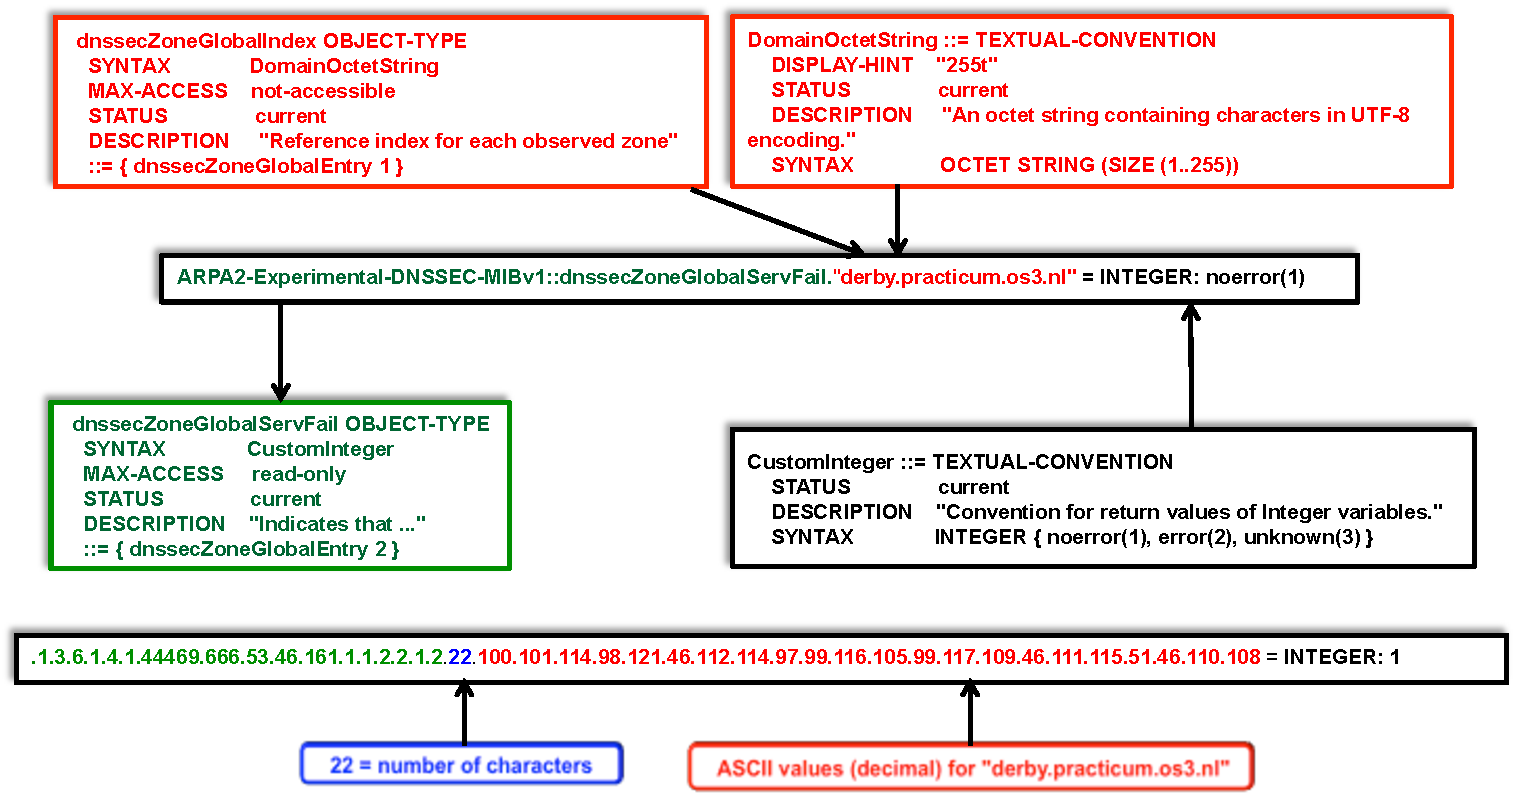
\includepdf[pages=-,scale=.7,pagecommand={}]{Images/tc1.pdf}
%%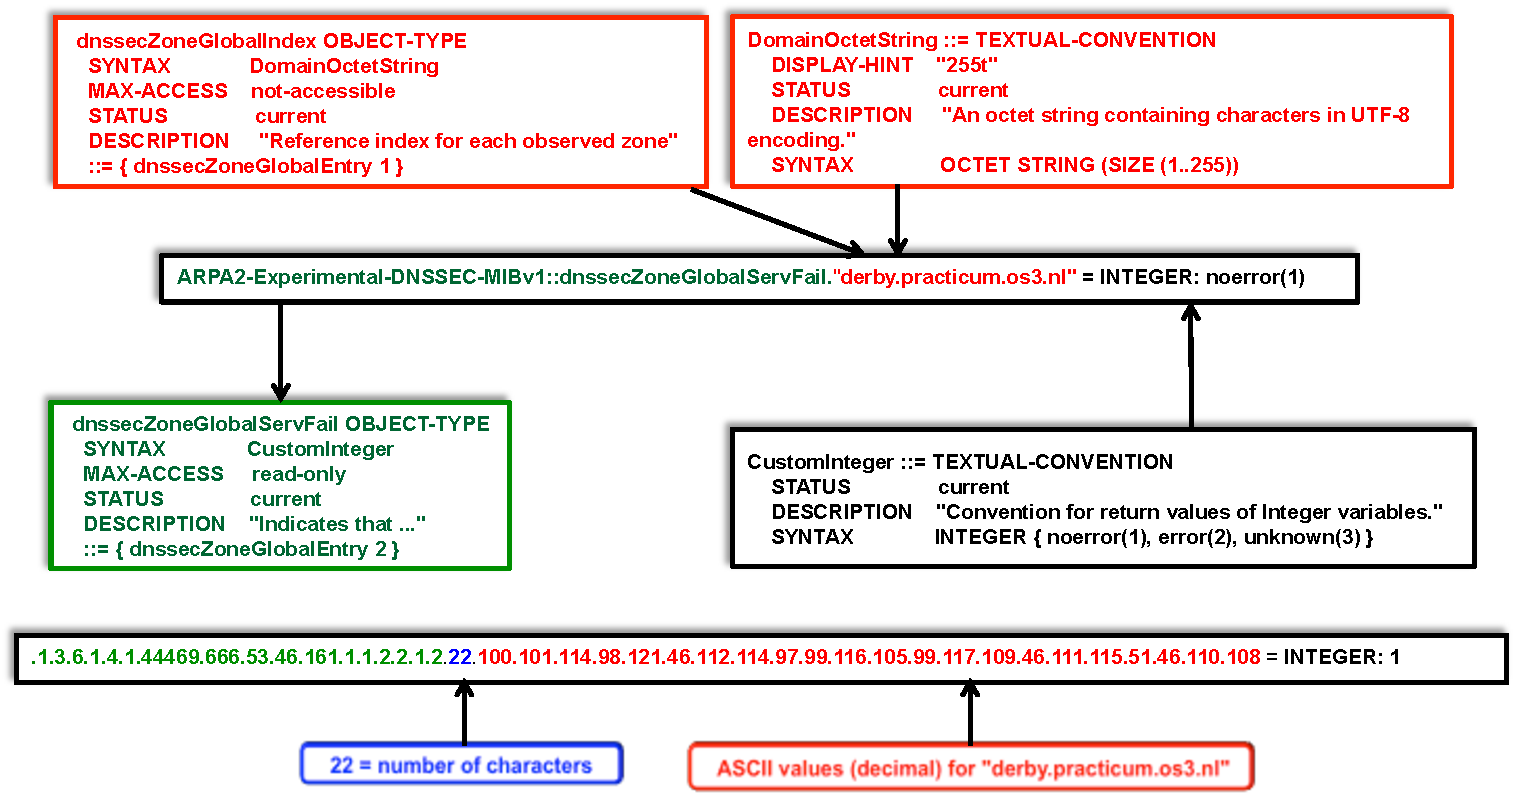
\includepdf[pages={1}]{Images/tc1.pdf}

\begin{figure}[htp] \centering{
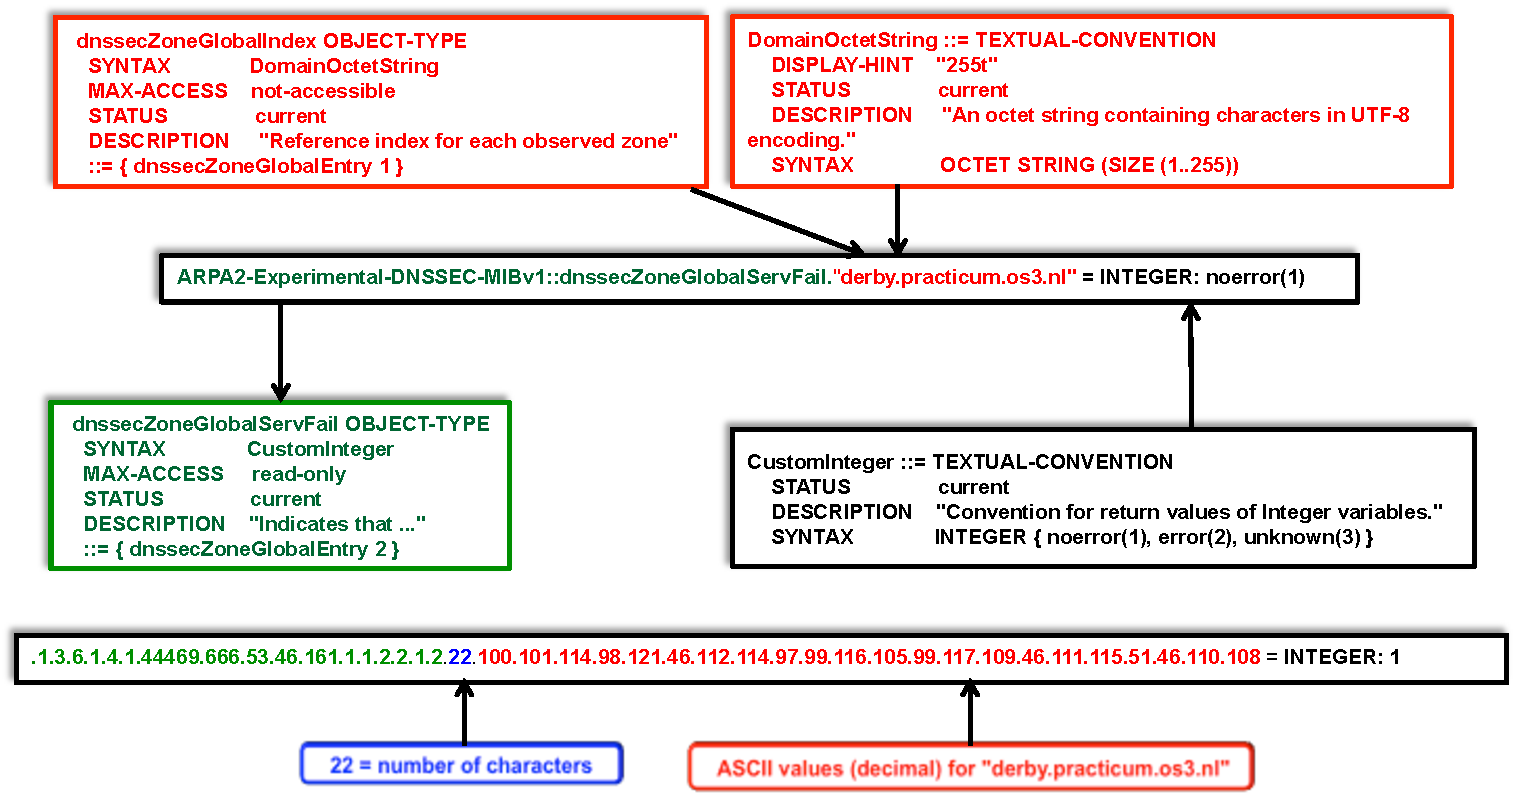
\includegraphics[scale=0.5]{Images/tc1.pdf}}
\caption{Effect of textual conventions to represent MIB data}
\label{figure:textual-conventions}
\end{figure}

A textual convention \textit{DomainOctetString} is defined and mapped to the \textit{dnssecZoneGlobalIndex}. That textual convention specifies the usage of the underlying datatype OCTET STRING and limits its number of octets to 255. That number represents the maximum allowed number of octets a domain name can contain \cite{wiki-domainnames}. Although the maximum allowed number of octets a domain name can contain is limited to 255, an IDNE proposal \cite{idne} (Internationalized domain names using EDNS) exists that uses the DNS extension mechanism called EDNS \cite{edns}. The extension allows some IDNE labels to be longer than 63 characters and some IDNE names to be longer than 255 octets. That would allow to send domain names either as ASCII or binary, and the binary format is UTF-8. The \textit{DISPLAY-HINT} clause specifies the usage of UTF-8 encoded characters \cite{smi-tc}. That string, which represents a domain name is appended as an index value to each instance of an object-type.
\\ 
The textual convention \textit{CustomInteger} restricts the values that object-type \textit{dnssecZoneGlobalServFail} can have. In that case we allow the values shown in table \ref{table-tc}. That enables us to implement our agent data wrapper scripts in a way that for each check only these values can occur and we can associate them to a textual equivalent. Figure \ref{figure:textual-conventions} also shows the numerical representation of an instance of object-type\textit{dnssecZoneGlobalServFail} and how the OID for the SNMP message is constructed on the wire. The green marked numbers are the numerical identifiers for the object-type itself. Then the number of characters of the associated index is appended to the OID and finally the ASCII values in decimal for each character of the domain name. 

\begin{table}[h]
   \centering
  \begin{tabular}{|c|c|}
  \hline
  \textbf{Value} & \textbf{Meaning} \\
  \hline
  1 & No error \\
  \hline
  2 & Error \\
  \hline
  3 & Unknown \\
  \hline  
\end{tabular} 
\caption{Textual convention for integer variables }
\label{table-tc}
\end{table}
 
